\documentclass[12pt, right open]{memoir}
\usepackage{graphicx}
\usepackage{tikz}
\usetikzlibrary{matrix,chains,positioning,decorations.pathreplacing,arrows,automata}
\usetikzlibrary{shapes.geometric, calc, intersections}
\usepackage{mathtools}
\usepackage{amsmath}
\usepackage{float}
\floatstyle{boxed}
\restylefloat{figure}
\usepackage{multirow} %for tables
\usepackage{ifthen}
\setcounter{secnumdepth}{5}

%To reduce vetical line spaces between list items
\usepackage{enumitem}
\setlist{nolistsep,leftmargin=*}

\newcommand{\specialcell}[2][c]{%
  \begin{tabular}[#1]{@{}c@{}}#2\end{tabular}}
%  Foo bar & \specialcell{Foo\\bar} & Foo bar \\    % vertically centered
%Foo bar & \specialcell[t]{Foo\\bar} & Foo bar \\ % aligned with top rule
%Foo bar & \specialcell[b]{Foo\\bar} & Foo bar \\ % aligned with bottom rule

\newcommand{\matplus}{
~~
  }

\begin{document}

%http://www.comp.leeds.ac.uk/ai23/reading/Hopfield.pdf

% >>>>>>>> Tikz Style sheet
\tikzstyle{every pin edge}=[<-,shorten <=1pt]
\tikzstyle{neuron}=[circle,fill=black!25,minimum size=17pt,inner sep=0pt]
\tikzstyle{input neuron}=[neuron, fill=black!50]
\tikzstyle{output neuron}=[neuron, fill=black!50]
\tikzstyle{hidden neuron}=[neuron, fill=black!50]
\tikzstyle{annot} = [text width=4em, text centered]

\tikzstyle{startstop} = [rectangle, rounded corners, minimum width=3cm, minimum height=1cm,text centered, draw=black]
\tikzstyle{io} = [trapezium, trapezium left angle=70, trapezium right angle=110, minimum width=3cm, minimum height=1cm, text centered, draw=black]
\tikzstyle{process} = [rectangle, minimum width=3cm, minimum height=1cm, text centered, text width=3cm, draw=black]
\tikzstyle{decision} = [diamond, minimum width=3cm, minimum height=1cm, text centered, draw=black]
\tikzstyle{arrow} = [thick,->,>=stealth]
% <<<<<<<< Tikz Style sheet

%%%%%%%%%%%%%%%%%%%%%%%%%%%%%%%%%%%%%%%%%%%%%%%%%%%%%%%%%%%%%%%%%%%%%%%%%%%%%%%%%%%%%%%%%%%
\chapter{Instrumentation, Measurement,
and Industrial Applications}

Instrumentation and measurement play a relevant role in any industrial applications.
Without sensors, transducers, converters, acquisition channels, signal processing, image
processing, no measurement system and procedure will exist and, in turn, no industry will
actually exist. They are in fact the irreplaceable foundation of any monitoring and
automatic control system as well as for any diagnosis and quality assurance.

A number of results concerning the use of neural techniques are known in
different applications, encompassing intelligent sensors and acquisition systems, system
models, signal processing, image processing, automatic control systems, and diagnosis.

\section{Fundamentals}
The concept of measurement has been deep-rooted in the human culture since the origin of
civilization, as it has always represented the basis of the experimental knowledge, the
quantitative assessment of goods in commercial transactions, the assertion of a right, and so
on.
After Galileo Galilei put experimentation at the base of the modern science and showed
that it is the only possible starting point for the validation of any scientific theory, the
measurement activity has become more and more important. More than one century ago,
William Thomson, Lord Kelvin, reinforced this concept by stating: \textbf{"I often say that when
you can measure what you are speaking about, and can express it in numbers, you know
something about it; but when you cannot express it in numbers your knowledge about it is
of meager and unsatisfactory kind; it may be the beginning of knowledge, but you have
scarcely, in your thoughts, advanced to the stage of science, whatever the matter may be.
So, therefore, if science is measurement, then without metrology there can be no science"}.


Under this modem vision of science, the measurement of a physical quantity is
generally defined as the quantitative comparison of this same quantity with another one,
which is homogeneous with the measured one, and is considered as the measurement unit.
In order to perform this quantitative comparison, five agents are needed,

\begin{itemize}
\item \textbf{The measurand}: it is the quantity to be measured, and it often represents a property of a
physical object and is described by a suitable mathematical model.
\item \textbf{The standard}: it is the physical realization of the measurement unit.
\item \textbf{The instrument}: it is the physical device that performs the comparison.
\item \textbf{The method}: the comparison between the measurand and the standard is performed by
exploiting some physical phenomena (thermal dilatation, mechanical force between
electric charges, and so on); according to the considered phenomenon, different methods
can be implemented.
\item \textbf{The operator}: he supervises the whole measurement process, operates the measurement
devices and reads the instrument.
\end{itemize}

\begin{figure}
\centering
\caption{Pictorial representation of Measurement}
\label{fig:pictorial_representation_of_measurement}
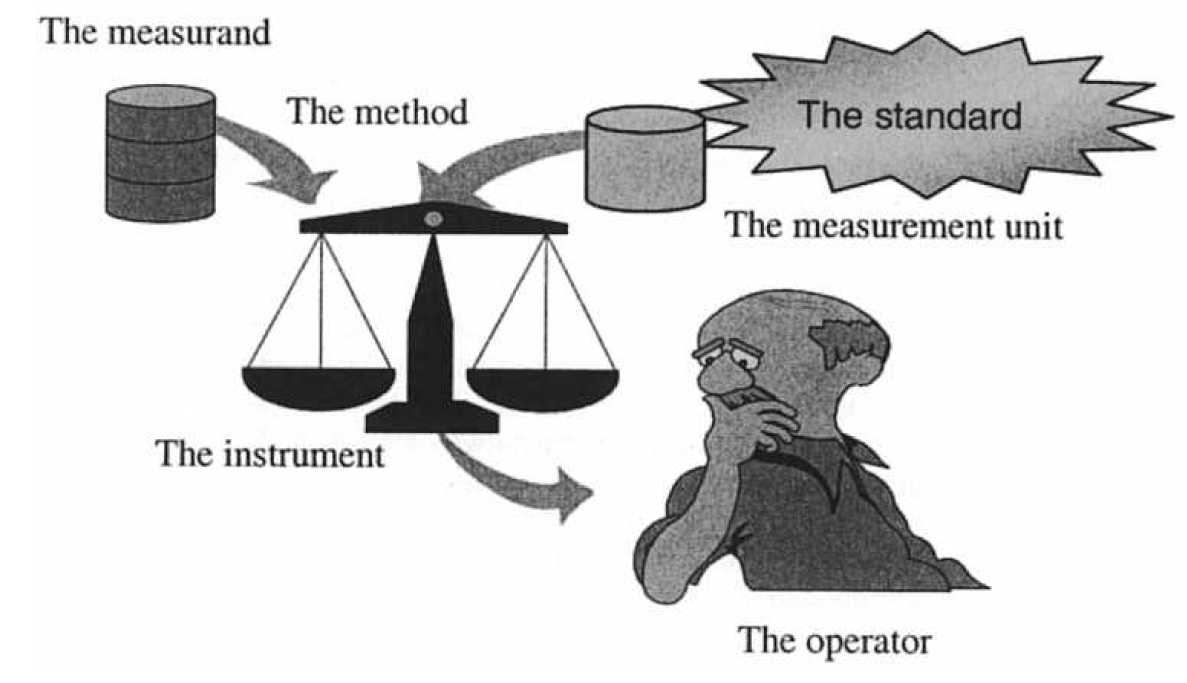
\includegraphics[scale=.5]{measurement.png}
\end{figure}

\end{document}